%%% Template originaly created by Karol Kozioł (mail@karol-koziol.net) and modified for ShareLaTeX use

\documentclass[a4paper,11pt]{article}

\usepackage[T1]{fontenc}
\usepackage[utf8]{inputenc}
\usepackage[francais]{babel}
\usepackage{graphicx}
\usepackage{xcolor}

\renewcommand\familydefault{\sfdefault}
\usepackage{tgheros}
\usepackage[defaultmono]{droidmono}

\usepackage{amsmath,amssymb,amsthm,textcomp}
\usepackage{enumerate}
\usepackage{multicol}
\usepackage{tikz}
\usepackage{media9}

\usepackage{url}
\usepackage{animate}
\usepackage{listings}


\usepackage{geometry}
\geometry{total={210mm,297mm},
left=25mm,right=25mm,%
bindingoffset=0mm, top=20mm,bottom=20mm}

\usepackage[colorlinks=false]{hyperref}
\linespread{1.3}

\newcommand{\linia}{\rule{\linewidth}{0.5pt}}

% custom theorems if needed
\newtheoremstyle{mytheor}
    {1ex}{1ex}{\normalfont}{0pt}{\scshape}{.}{1ex}
    {{\thmname{#1 }}{\thmnumber{#2}}{\thmnote{ (#3)}}}

\theoremstyle{mytheor}
\newtheorem{defi}{Definition}

% my own titles
\makeatletter
\renewcommand{\maketitle}{
\begin{center}
\vspace{2ex}
{\huge \textsc{\@title}}
\vspace{1ex}
\\
\linia\\
\@author \hfill \@date
\vspace{4ex}
\end{center}
}
\makeatother
%%%
\usepackage{lastpage}
% custom footers and headers
\usepackage{fancyhdr}
\pagestyle{fancy}
\lhead{}
\chead{}
\rhead{}
\lfoot{L3 MIASHS - Web2}
\cfoot{}
\rfoot{Page \thepage/\pageref{LastPage}}
\renewcommand{\headrulewidth}{0pt}
\renewcommand{\footrulewidth}{0pt}
%
%%%----------%%%----------%%%----------%%%----------%%%
\usepackage{xcolor}

\colorlet{punct}{red!60!black}
\definecolor{background}{HTML}{EEEEEE}
\definecolor{delim}{RGB}{20,105,176}
\colorlet{numb}{magenta!60!black}

\lstdefinelanguage{json}{
    basicstyle=\scriptsize\ttfamily,
    numbers=left,
    numberstyle=\scriptsize,
    stepnumber=1,
    numbersep=8pt,
    showstringspaces=false,
    breaklines=true,
    frame=lines,
    backgroundcolor=\color{background},
    literate=
     *{0}{{{\color{numb}0}}}{1}
      {1}{{{\color{numb}1}}}{1}
      {2}{{{\color{numb}2}}}{1}
      {3}{{{\color{numb}3}}}{1}
      {4}{{{\color{numb}4}}}{1}
      {5}{{{\color{numb}5}}}{1}
      {6}{{{\color{numb}6}}}{1}
      {7}{{{\color{numb}7}}}{1}
      {8}{{{\color{numb}8}}}{1}
      {9}{{{\color{numb}9}}}{1}
      {:}{{{\color{punct}{:}}}}{1}
      {,}{{{\color{punct}{,}}}}{1}
      {\{}{{{\color{delim}{\{}}}}{1}
      {\}}{{{\color{delim}{\}}}}}{1}
      {[}{{{\color{delim}{[}}}}{1}
      {]}{{{\color{delim}{]}}}}{1},
}

%\begin{filecontents}{timeline.txt}
%::0x0 % coordinate system & y=e^x, repeated until last frame
%::1 % one blue curve per frame
%::2
%::3
%::4
%::5
%::6
%::7
%::8
%\end{filecontents}

\begin{document}

\title{TP 2 - Mémo LoL (part 1)}

\author{Université Toulouse 2 - Jean Jaurès}

%\date{01/01/2014}

\maketitle
\tableofcontents

\section*{Présentation du TP}
Dans ce TP vous allez devoir réaliser un jeu de memory avec le framework CSS Bootstrap (v3.3.7) et le pré-processeur CSS Less.js (v2.7.2) en utilisant les données du jeu League Of Legends (LoL) dont la présentation du jeu est disponible \href{http://euw.leagueoflegends.com/fr}{ici}\footnote{\url{http://euw.leagueoflegends.com/fr}}.

LoL propose à 10 joueurs de s'affronter en 5 contre 5, chacun incarnant un champion et devant protéger une base tout en essayant de détruire la base ennemie. Riot Games\textsuperscript{\texttrademark} (l'entreprise qui a créé ce jeu) a mis à disposition une API (\textit{Application Programming Interface} ou Interface de Programmation)  pour récupérer les données du jeu, notamment les données concernant les champions disponibles. Nous proposons ici de développer le jeu du memory en utilisant ces données pour que les cartes représentent des champions du jeu LoL. 

Le jeu du memory consiste à avoir un nombre paire de cartes faces cachées présentées au joueur. Celui-ci doit retrouver les paires de cartes correspondantes. Pour cela il peut retourner simultanément 2 cartes. Si celles ci correspondent (le nom du champion est le même) alors la paire reste retournée. Sinon les deux cartes sont remises faces cachées et le joueur tente de retourner une autre paire de cartes. Le jeu se terminer lorsque toutes les paires sont trouvées. \\


\begin{center}

\includegraphics[width=0.2\textwidth]{img/lol.png} \\
%
\includegraphics[width=0.05\textwidth]{img/UOL_logo.png}
\end{center}

\section{Interface}
Cette première partie se concentre sur la mise en place de l'interface statique de l'application. Il faut d'abord créer un plateau de jeu avec des cartes pré-sélectionnées et ensuite créer les animations qui seront utilisées pendant le déroulement de la partie. Seuls HTML et CSS seront utilisés pour cela. 

\subsection{Mise en place de l'interface}
\subsubsection{Cartes de champions}
En utilisant les frameworks Bootstrap\footnote{\url{https://getbootstrap.com/}} et LESS\footnote{\url{http://lesscss.org/}} vus en cours, vous devez mettre en place l'interface présentant le plateau de jeu. Ce plateau comprend 3 cartes représentant 3 champions de LoL. Pensez à utiliser le système de "grid" de Bootstrap pour rendre votre application \textit{responsive}. Vous utiliserez les liens suivant pour les images : 
\small
\begin{itemize}
    \item \url{https://ddragon.leagueoflegends.com/cdn/img/champion/splash/Ivern_0.jpg}
    \item \url{https://ddragon.leagueoflegends.com/cdn/img/champion/splash/Teemo_0.jpg}
    \item \url{https://ddragon.leagueoflegends.com/cdn/img/champion/splash/Taric_0.jpg}
\end{itemize}
\normalsize
Vous devez obtenir le plateau suivant : \\
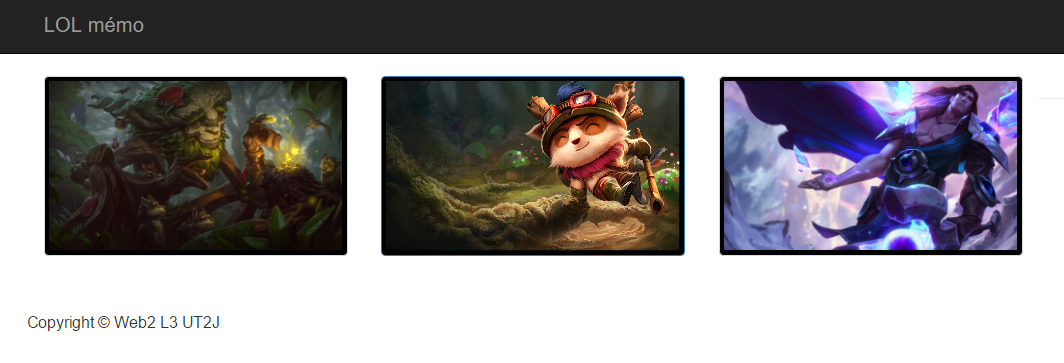
\includegraphics[width=\textwidth]{img/plateau.png}

\subsubsection{Paire de cartes}
De la même manière, rajoutez 3 cartes correspondantes à ces cartes. Pour cela vous utiliserez une autre image du même champion en remplaçant le "\_0" à la fin du nom du fichier par un "\_1" \footnote{Par exemple \url{https://ddragon.leagueoflegends.com/cdn/img/champion/splash/Ivern_1.jpg}}. Afin de permettre l'identification du héro (qui n'est pas toujours évidente sur les images) vous rajouterez le nom du champion en dessous de l'image. Vous obtenez alors le rendu suivant : \\
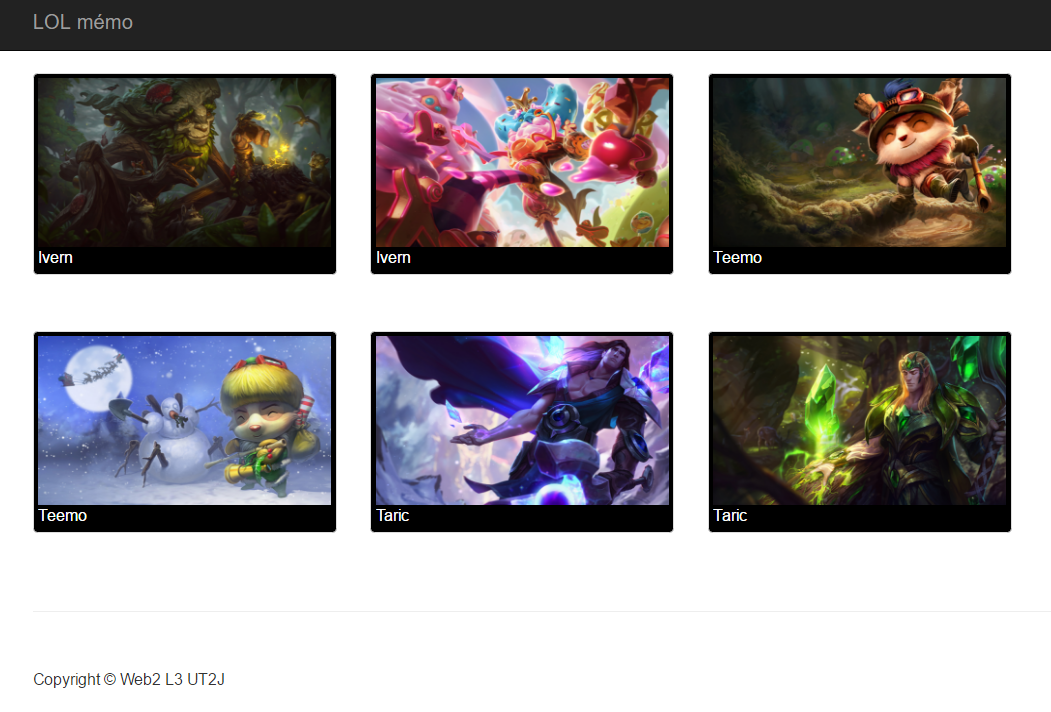
\includegraphics[width=\textwidth]{img/plateau2.png}

\subsubsection{Dos des cartes}
Par défaut les cartes sont affichées face cachée. Pour cela il faut donc afficher une image par défaut (de votre choix) et afficher la carte (et le nom) du champion que lorsque la souris survol la carte. Comme l'exemple suivant : \\
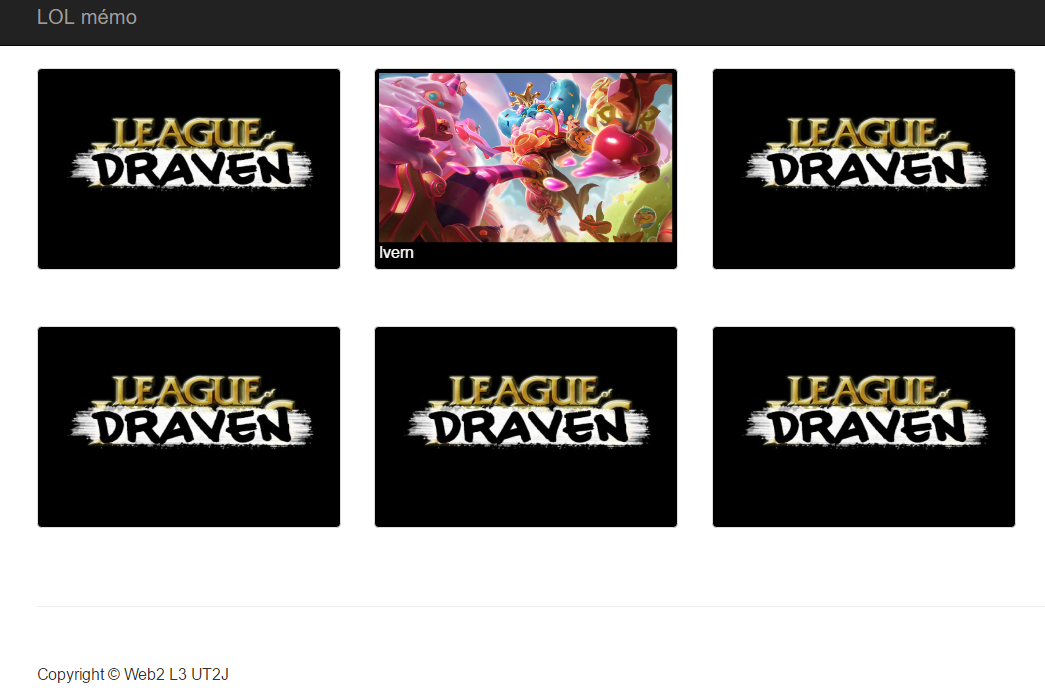
\includegraphics[width=\textwidth]{img/plateau3.png}

\subsection{Animations CSS3}
\subsubsection{Animation des cartes}
Dans cette partie nous allons utiliser les fonctionnalités du CSS3 afin de générer une animation pour simuler l'effet de "retournement d'une carte"\footnote{Indice : \url{http://www.w3schools.com/css/css3_3dtransforms.asp}}. Exemple : \\
%\animategraphics[loop, autoplay, controls, width=\textwidth]{5}{img/animation/output-}{10}{17}

   % \animategraphics[
    %label=taylor, autoplay, loop, width=\textwidth,
%    timeline=timeline.txt
 %   ]{1}{./img/animation/output-}{12}{17}
    % \mediabutton[
    % jsaction={
    % if(anim[’taylor’].isPlaying)
    % anim[’taylor’].pause();
    % else
    % anim[’taylor’].playFwd();
    % }
    % ]{\fbox{Play/Pause}}


	\animategraphics[autoplay,loop,width=\textwidth,controls]{3}{img/animation/output-}{0}{17} 

\subsubsection{Animation du plateau (Bonus)}
Faire une animation d'introduction du plateau. Par exemple animez les cartes pour simuler leur arrivé par la gauche. Soyez créatif! 


\end{document}
